%styl klasy z Polskimi Normami oprac. Marcin Wolinski
\documentclass[a4paper, titleauthor]{mwart} 

\usepackage{polski}
\usepackage[utf8]{inputenc}
\usepackage{graphicx} %pakiet do wstawiania grafiki
\usepackage[hyphens]{url} %pakiet do wstawiania linkow
%\usepackage[hidelinks,breaklinks]{hyperref}
\usepackage{authblk}%pakiet do tworzenia afiliacji
\usepackage{tabularx}%pakiet do tabel
\usepackage[a4paper, left=2cm, right=2cm, top=3cm, bottom=3cm]{geometry}
\usepackage{listings}
\usepackage{placeins}%pakiet do kontroli umieszczania obiektow
\usepackage{hyperref}%pakiet do m.in. kolorowania linkow
\usepackage{subcaption}
\usepackage[tablegrid,owncaptions]{vhistory}
\renewcommand{\vhhistoryname}{Historia zmian}
\renewcommand{\vhversionname}{Wersja}
\renewcommand{\vhdatename}   {Data}
\renewcommand{\vhauthorname} {Autor}
\renewcommand{\vhchangename} {Opis zmian}

\renewcommand\figurename{Rys.}%skrocony podpis
\renewcommand\lstlistingname{Wydruk}
\lstset{
backgroundcolor=\color{white},
showspaces=false,
showstringspaces=false,
showtabs=false,
frame=single,
tabsize=2,
captionpos=b,
breaklines=true,
breakatwhitespace=false,
breakautoindent=true,
escapeinside={\%*}{*)},
linewidth=\textwidth,
escapechar=\&,
escapeinside={(*@}{@*)},
}
\hypersetup{
    colorlinks=true,
    linkcolor=blue,
    filecolor=magenta,      
    urlcolor=cyan,
    pdftitle={Overleaf Example},
    pdfpagemode=FullScreen,
}

\title{{\Huge  Projekt SYCYF}\\ - \\{\Large Zespół nr 2}\\ }

\author{Artur Hrianka \and Ernest Korotkov \and Michał Sokala \and Michał Krzyżanowski \and Wiktor Frątczak}

\affil{Politechnika Warszawska, Instytut Telekomunikacji}
\date{\today}

%------------------------------------------------------------------------
% Początek dokumentu
\begin{document}

%Automatycznie generowany tytuł dokumentu
\maketitle
%podpis na dole strony, bez numeru

%------------------------------------------------------------------------
% Historia zmian
\begin{versionhistory}
	\vhEntry{1.0}{12.03.2023}{AH|EK|MS|MK|WF}{Pierwsza wersja raportu}
       \vhEntry{1.1}{13.03.2023}{EK|AH|MS|MK|WF}{Opis narzędzi do pracy nad projektem}
       \vhEntry{2.0}{02.04.2023}{EK|AH|WF|MS|MK}{Wyszukiwanie artykułów i publikacji w zakresie naszego projektu; zapoznanie się z teorią, niezbędną do realizacji projektu; poszukiwanie istniejących rozwiązań; wybór narzędzi}
       \vhEntry{2.1}{03.04.2023}{EK|AH|WF|MS|MK}{Umieszczenie informacji znalezionych przez nasz zespół do dokumentu z sprawozdaniem wraz z bibliografią}
       \vhEntry{2.2}{04.04.2023}{EK|AH|WF|MS|MK}{Finalizacja etapu II}
       \vhEntry{3.0}{15.04.2023}{EK|AH|WF|MS|MK}{Pierwsza wersja etapu III}
       \vhEntry{3.1}{17.04.2023}{EK|AH|WF|MS|MK}{Dalsza część prac nad etapem III}
       \vhEntry{3.2}{22.04.2023}{EK|AH|WF|MS|MK}{Finalizacja etapu III}
       \vhEntry{4.0}{18.05.2023}{EK|AH|WF|MS|MK}{Początek pracy nad etapem IV; pierwsze kroki w napisaniu programu w języku Verilog HDL}
       \vhEntry{4.1}{20.05.2023}{EK|AH|WF|MS|MK}{Modyfikacja naszego kodu; pierwsze testy na poprawność działania}
       \vhEntry{4.2}{22.05.2023}{EK|AH|WF|MS|MK}{Słowny opis realizacji etapu; kończenie pracy nad kodem}
       \vhEntry{4.3}{23.05.2023}{EK|AH|WF|MS|MK}{Finalizacja etapu IV}
       \vhEntry{5.0}{6.06.2023}{EK|AH|WF|MS|MK}{Realizacja naszej sieci neuronowej z pomocą narzędzia Logisim}
       \vhEntry{5.1}{17.06.2023}{EK|AH|WF|MS|MK}{Wnoszenie poprawek do wszystkich etapów}
       \vhEntry{5.2}{18.06.2023}{EK|AH|WF|MS|MK}{Opis uruchomienia naszego projektu na płytce; finalizacja projektu}
\end{versionhistory}

%------------------------------------------------------------------------
% Automatycznie generowany spis treści
\tableofcontents

%------------------------------------------------------------------------
\section{\large Wstęp}
\label{sec:wstep}%etykieta

Celem projektu jest zbudowanie systemu rozpoznawania wzorców, który na wejściu otrzymuje wektor binarny reprezentujący piksele ramki o rozmiarach 4x4 piksele. System ten będzie mógł być wykorzystany w różnych dziedzinach, takich jak rozpoznawanie obrazów, identyfikacja znaków czy analiza sygnałów. Ten system będzie w stanie rozpoznawać znaczki "X" oraz "O", przy czym będzie uwzględniona możliwość zaszumienia obrazu. Projekt jest podzielony na kolejne etapy:

\renewcommand{\labelenumi}{\Roman{enumi}}
\begin{enumerate}\setlength{\itemsep}{0.2\baselineskip} 
	\item Etap wstępny – stworzenie zespołu i organizacja warsztatu pracy, 
	\item Etap zdobywania informacji – analiza literatury, istniejących metod, zebranie wiedzy teoretycznej związanej z tematem projektu, 
	\item Etap opracowania koncepcji – szukanie rozwiązań, najlepiej sprawdzi się proces burzy mózgów (mapy myśli), opracowanie koncepcji rozwiązania  na podstawie zdobytej wiedzy, opracowanie prostego modelu referencyjnego (Python, MATLAB/GNU Octave, itp) i danych do testowania  
	\item Etap implementacji – na tym etapie rozwijamy i rozbudowujemy koncepcje projektowe docelowego systemu, modelujemy elementy systemu w HDL, weryfikujemy funkcjonalnie, integrujemy i oceniamy prototypy, 
	\item Etap uruchomienia – wdrożenie projektu, uruchomienie na docelowej platformie, przetestowanie według wcześniej opracowanych scenariuszy testowych. 
 \newline
 \newline
\end{enumerate}
\section{\large Etap I}


\label{sec:organizacja}

\subsection{Design Thinking}
\label{sec:design_thinking}
Pięcioetapowy model Design Thinking- jeden z najpopularniejszych modeli, który składa się z 5 etapów: empatia, diagnoza potrzeb, generowanie pomysłów, prototypowanie i testowanie.
\begin{figure}[h]
\centering
    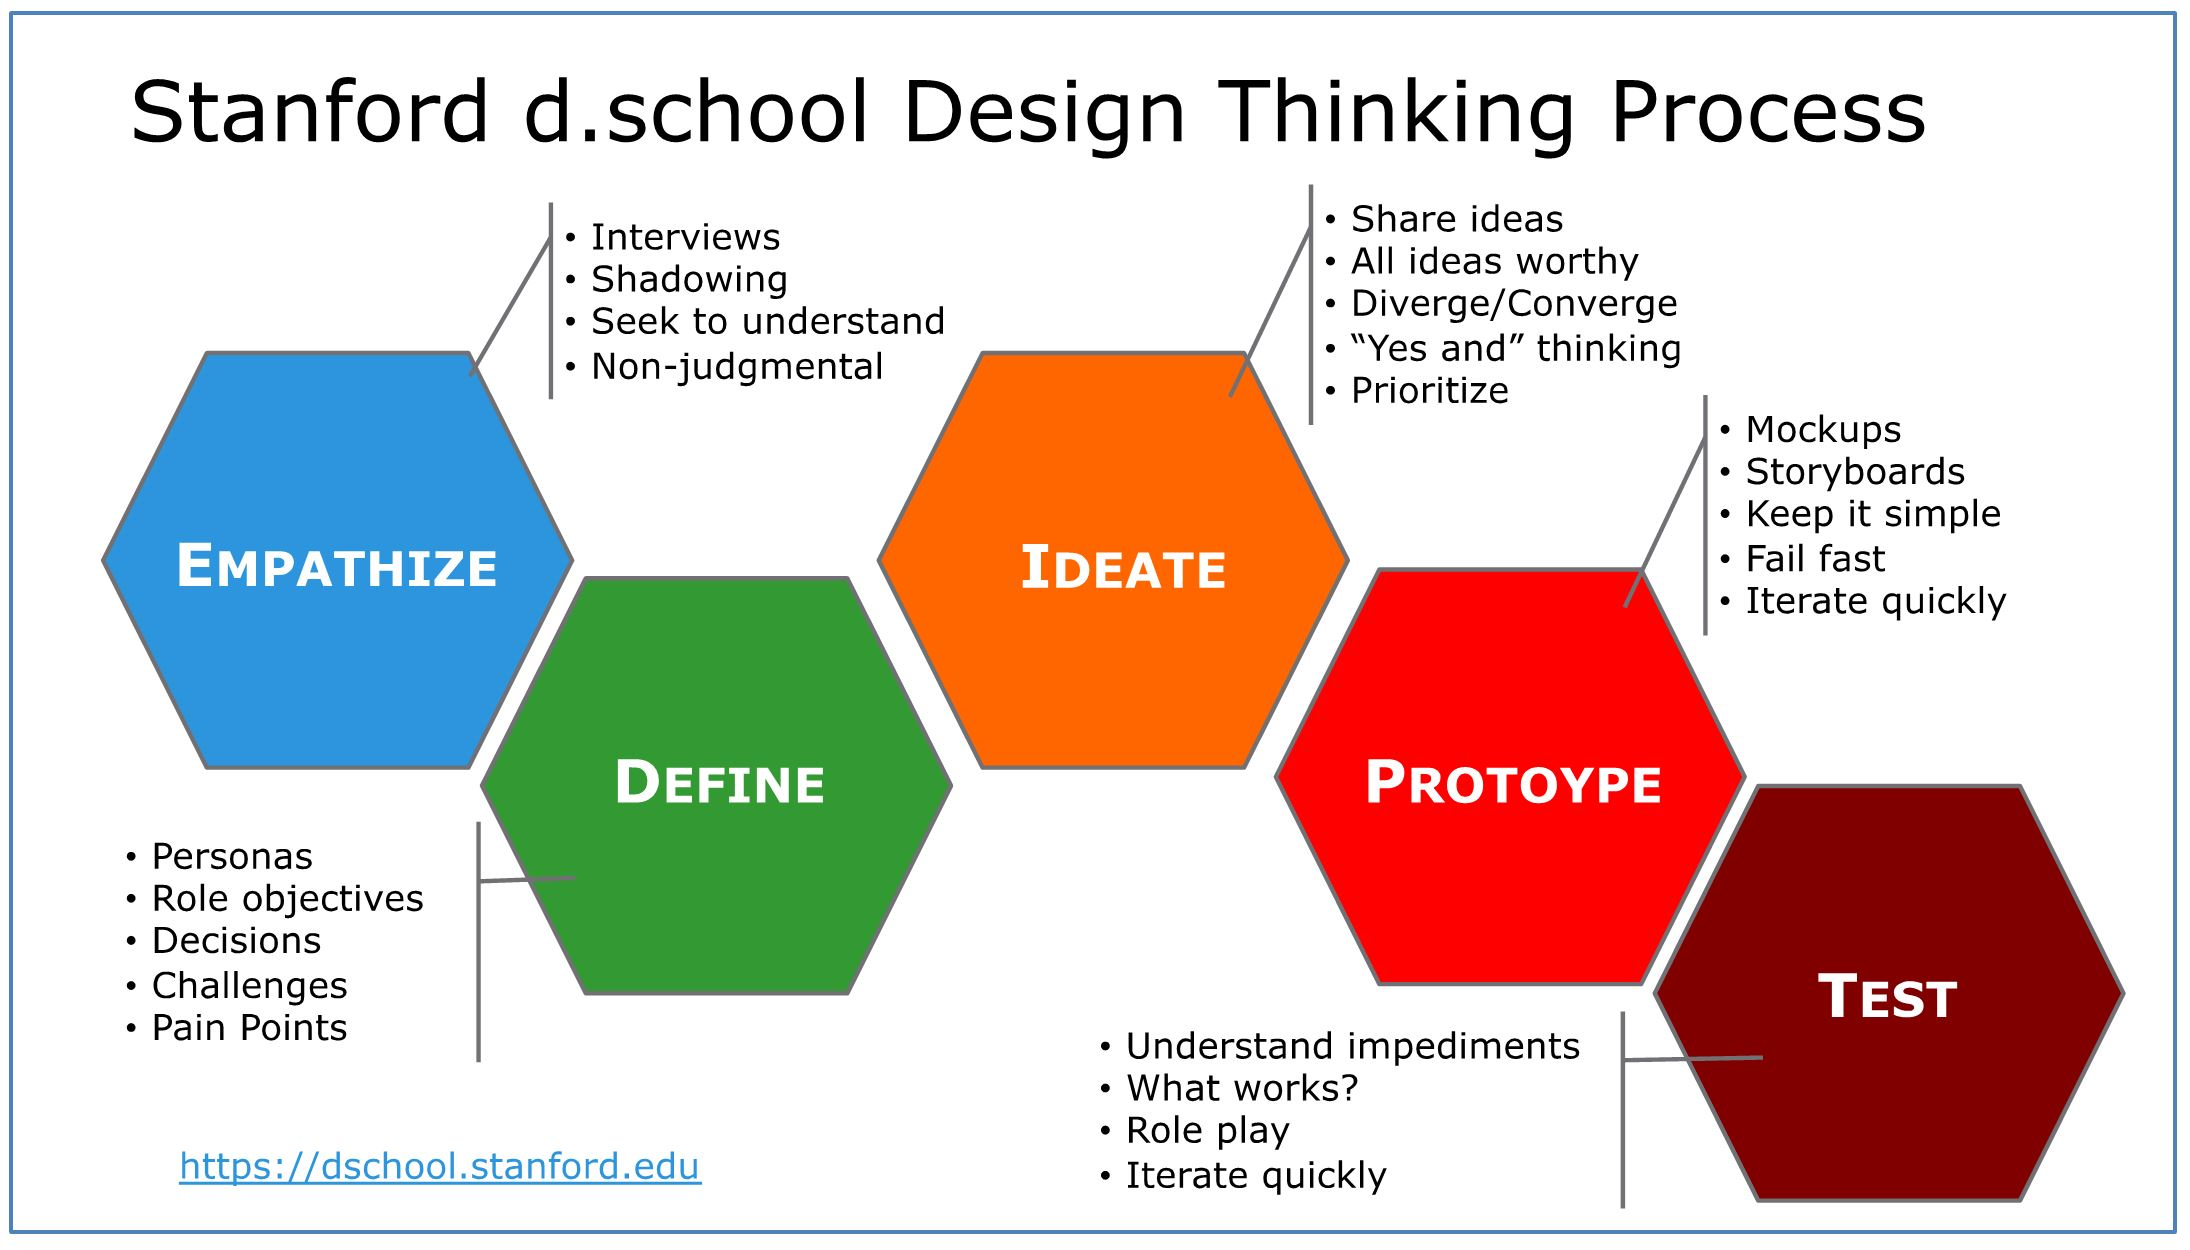
\includegraphics[width=0.8\linewidth]{Stanford-Design-Thinking-Process.jpg}
    \caption{Stanford Design Thinking}
\end{figure}

\subsection{Zarządzanie projektem}
\label{sec:zarządzanie_projektem}
\begin{figure}[h]
\centering
    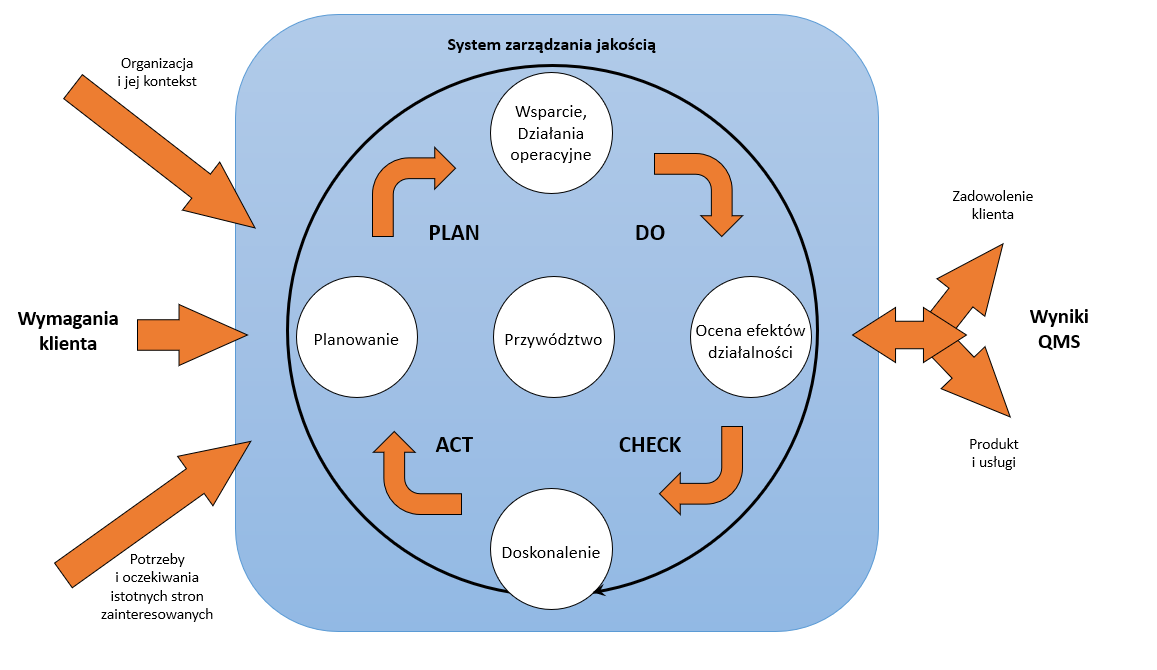
\includegraphics[width=0.8\linewidth]{Zarzadzanie.png}
    \caption{Zarządzanie projektem}
\end{figure}
Podczas zarządzania projektem, będziemy kierować się wspólnym podejmowaniem decyzji, oraz równym rozkładem obowiązków tak aby każdy wykonał podobną część projektu.
\subsubsection{Metoda Scrum}
Scrum to jedna z metodyk zwinnych(agile).Opisuje ona ramy procesu (framework) działania zespołów, które mają za zadanie wytworzyć i dostarczyć klientowi określony produkt.Pierwotnie scrum został stworzony dla pracowników działów IT, ale obecnie metodyka ta stosowana jest uniwersalnie.

Scrum  dość szczegółowo opisuje rozkład zadań — od planowania po dostarczenie gotowego produktu. To dlatego praca podzielona jest na odcinki takie jak:planowanie sprintu, daily scrum meetings, sprint review oraz sprint retrospective. 

Warto dodać, że najważniejsza w metodologii scrum jest przejrzystość. Informacja zwrotna na temat przebiegu pracy — bez względu na to, czy realizacja zadań przebiega pomyślnie, czy nie — jest kluczem do osiągnięcia pożądanego efektu. 

Podejmowanie decyzji według zasad scrum odbywa się na podstawie feedbacku otrzymywanego od poszczególnych zespołów i ich członków. W ten sposób można stale trzymać rękę na pulsie i kontrolować przebieg pracy.

\subsubsection{Narzędzia}
\label{sec:narzędzia}
\begin{enumerate}\setlength{\itemsep}{0.2\baselineskip} 
	\item Overleaf – edytor LaTeX online, który wykorzystamy do pisania sprawozdań 
	\item Microsoft Teams – szybka forma kontaktu z członkami zespołu i prowadzącymi 
	\item Google – wyszukiwarka dla znalezienia potrzebnych informacji
	\item PyCharm – najlepsze środowisko do pisania w języku Python 
	\item Intel Quartus – środowisko do realizacji naszego projektu w języku Verilog HDL
        \item GITLAB - VCS, repozytorium do, którego będziemy dodawać materiały potrzebne do realizacji projektu
\end{enumerate}
\newpage

\section{\large Etap II}

\subsection{Podstawowe informacje}
Rozpoznawanie wzorców(patter recognition) jest procesem, który polega na rozpoznawaniu cech szczególnych oraz prawidłowości obrazów lub sygnałów.
W projekcie realizacji systemu rozpoznawania wzorców otrzymującego na wejściu wektor binarny reprezentujący piksele ramki o rozmiarach 4×4 piksele, wymagana jest znajomość wielu informacji teoretycznych, narzędzi, a także istniejących rozwiązań.
\subsection{Publikacje wykorzystane podczas realizacji etapu II}

\begin{itemize}\setlength{\itemsep}{0.2\baselineskip}
    \item \href{https://www.microsoft.com/en-us/research/uploads/prod/2006/01/Bishop-Pattern-Recognition-and-Machine-Learning-2006.pdf}{"Pattern Recognition and Machine Learning"} autorstwa Christophera Bishopa. W publikacji tej omówiono wiele algorytmów i technik wykorzystywanych w rozpoznawaniu wzorców, takich jak sieci neuronowe czy algorytmy k-najbliższych sąsiadów. 
\newline
    \item \href{https://www.irjet.net/archives/V4/i7/IRJET-V4I7599.pdf}{"Handwritten Digit Recognition using Convolutional Neural Networks"} autorstwa Yann LeCun, który przedstawiał zastosowanie sieci neuronowych w rozpoznawaniu ręcznie pisanych cyfr.
\newline
	\item \href{https://arxiv.org/pdf/1512.03385.pdf}{"Deep Residual Learning for Image Recognition"} autorstwa K. He, X. Zhang, S. Ren i J. Sun opisuje model głębokiej sieci neuronowej nazwanej ResNet. Autorzy wprowadzili pojęcie bloków rezydualnych, które pozwalają na sprawniejsze trenowanie sieci o dużych głębokościach, jednocześnie zapobiegając problemowi degradacji dokładności wraz ze wzrostem liczby warstw. ResNet osiągnął najlepsze wyniki w wielu popularnych zbiorach danych.
\newline
    \item \href{https://www.researchgate.net/publication/220651964_An_Overview_of_Pattern_Recognition_Techniques}{"An Overview of Pattern Recognition Techniques"} autorstwa L. Rokach i O. Maimon, opublikowany w czasopiśmie "Journal of Information Science and Engineering". W artykule tym opisane są różne metody rozpoznawania wzorców, takie jak sieci neuronowe, drzewa decyzyjne, algorytmy genetyczne i wiele innych.
\newline
    \item \href{https://darmanto.akakom.ac.id/pengenalanpola/Pattern%20Recognition%204th%20Ed.%20(2009).pdf}{"A review of pattern recognition techniques"} autorstwa S. Theodoridis i K. Koutroumbas, opisujące podstawowe techniki rozpoznawania wzorców, takie jak klasyfikacja liniowa, klasyfikacja nieliniowa, sieci neuronowe i drzewa decyzyjne.
\newline
    \item \href{https://kgut.ac.ir/useruploads/1550563201478ety.pdf}{"Image Processing, Analysis, and Machine Vision"} to obszerna książka poświęcona tematyce przetwarzania obrazów, analizy obrazów oraz widzenia maszynowego. Książka zawiera szeroki wachlarz technik i metod związanych z rozpoznawaniem obiektów, segmentacją obrazów, klasyfikacją obrazów, analizą tekstury, uczeniem maszynowym i wieloma innymi zagadnieniami.
 
\end{itemize}

\subsection{Istniejące rozwiązania}
Na rynku dostępnych jest wiele gotowych rozwiązań do rozpoznawania wzorców, takich jak biblioteki OpenCV, TensorFlow czy Keras. Te narzędzia oferują wiele funkcjonalności związanych z przetwarzaniem obrazów oraz uczeniem maszynowym, co ułatwia proces tworzenia systemów rozpoznawania wzorców:
\newline
\begin{itemize}
    \item Jednym z popularnych modeli konwolucyjnych sieci neuronowych jest model LeNet-5\hyperref[1]{[1]}, który został opracowany w latach 90-tych przez Y. LeCun'a i jego zespół. LeNet-5 składa się z kilku warstw konwolucyjnych oraz warstw poolingowych. Modele tego typu są często stosowane do rozpoznawania odręcznie pisanych cyfr.
\newline
    \item Innym popularnym modelem konwolucyjnej sieci neuronowej jest model ResNet\hyperref[2]{[2]}, który został zaproponowany przez K. He i jego zespół w 2015 roku. Model ResNet wyróżnia się wykorzystaniem bloków rezydualnych, które pozwalają na bardziej efektywną naukę sieci neuronowej.
\newline
    \item Metoda k-najbliższych sąsiadów (k-NN)\hyperref[3]{[3]} - polega na znajdowaniu k najbliższych wzorców w zbiorze treningowym i klasyfikowaniu obiektu na podstawie etykiet tych wzorców. Ta metoda jest stosunkowo prosta, ale może być skuteczna w niektórych przypadkach.
\newline
    \item Sieci neuronowe - są to modele matematyczne, które naśladują sposób działania ludzkiego mózgu. Mogą być stosowane do rozpoznawania wzorców w obrazach i tekstach. Do trenowania sieci neuronowych można wykorzystać algorytmy uczenia nadzorowanego lub nienadzorowanego. 
\newline
    \item Segmentacja obrazu: Jest to proces podziału obrazu na mniejsze części, takie jak regiony, krawędzie i kontury, które są prostsze do przeanalizowania. Segmentacja obrazu może być stosowana do wyodrębnienia obiektów z tła na obrazie. Przykładowe metody segmentacji obejmują segmentację progową, segmentację opartą na kolorze, segmentację opartą na teksturze i segmentację opartą na konturach.
\newline
    \item Klasyfikacja obrazów: Ta metoda polega na przypisaniu obrazów do różnych klas lub kategorii na podstawie ich właściwości. W przypadku rozpoznawania obiektów, klasyfikacja obrazów może być wykorzystana do rozpoznawania obiektów na podstawie ich kształtu, tekstury, barwy i innych właściwości. Klasyfikacja może być oparta na różnych algorytmach, takich jak algorytm k-NN, SVM\hyperref[4]{[4]}, drzewa decyzyjne i sieci neuronowe.
\newline
    \item Wzorce Haar'a- Wzorce Haar'a są matematycznymi wzorcami, które mogą być wykorzystane do detekcji krawędzi i innych cech w obrazach.  Są one często stosowane w systemach rozpoznawania twarzy. Do wykrywania cech obiektów na obrazach, wzorce Haar'a są przesuwane po obrazie, a wynikiem jest obraz cech, który zawiera informacje o tym, gdzie na obrazie występują te cechy.
\newline
    \item Analiza tekstury- Ta metoda polega na analizie cech tekstury obiektów na obrazie, takich jak ziarnistość, szorstkość, kierunek i regularność. Analiza tekstury może być używana do rozpoznawania różnych obiektów, takich jak kamienie, drewno czy tkaniny. W celu analizy tekstury, obraz jest dzielony na mniejsze obszary, a następnie obliczane są statystyki tekstury, takie jak histogramy, spektra mocy oraz macierze współczynników.
\newline 
    \item Template matching- Jest jedną z najbardziej popularnych metod porównywania obrazów jest metoda porównywania ze wzorcem piksel po pikselu. Jest to metoda dość mało efektywna w związku z czym jest stosowana do obrazów o małych rozmiarach.\hyperref[5]{[5]}
\newline
\end{itemize}

\subsection{Informacje teoretyczne niezbędne do realizacji projektu}
Do realizacji projektu niezbędne są podstawowe informacje związane z przetwarzaniem obrazów, takie jak: reprezentacja obrazu w postaci macierzy pikseli, metody przetwarzania obrazów (filtracja, segmentacja, wyostrzanie, itp.), reprezentacja kolorów oraz metody uczenia maszynowego, takie jak sieci neuronowe czy metoda SVM.
\subsection{Narzędzia, które zostaną użyte do realizacji projektu}
Do realizacji projektu zostaną wykorzystane narzędzia takie jak: język programowania Python, biblioteki NumPy i SciPy do przetwarzania danych, biblioteka TensorFlow do uczenia maszynowego oraz środowisko Jupyter Notebook do tworzenia notatek i eksperymentów. 
W ramach projektu będziemy korzystać z oprogramowania Quartus do implementacji algorytmu w układzie, a także z narzędzi Matlab i Octave do analizy wyników i testowania algorytmu. Quartus jest popularnym narzędziem do projektowania i implementacji cyfrowych układów logicznych, a Matlab i Octave są narzędziami do obliczeń numerycznych i analizy danych, które są często stosowane w dziedzinie uczenia maszynowego.
\subsection{Wnioski}
Po wspólnych poszukiwaniach, research'u, wielokrotnych rozmowach oraz  zastosowaniu się do sugestii prowadzącego doszliśmy do wniosku, że do postawionego problemu projektowego, w którym musimy uwzględnić możliwe zniekształcenia w otrzymanych danych wejściowych, najłatwiej i najefektywniej będzie wykorzystać sieć neuronową typu MLP. 

\newpage
\section{\large Etap III}
\subsection{Schemat blokowy oraz jego omówienie + Proste zilustrowanie działania}


Przygotowaliśmy wektory binarne o długoci 16, które nie były wykorzystane w procesie treningowym.


\begin{figure}[h]
    \centering
    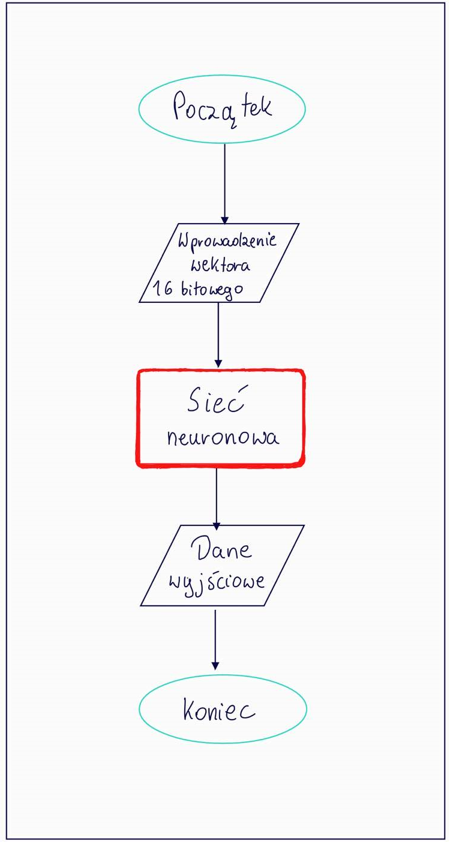
\includegraphics[width=1\linewidth, height=1\linewidth]{schemat_blokowy.png}
    \caption{Schemat blokowy}
\end{figure}
Podczas procesu propagacji sygnału w sieci neuronowej, każde wejście jest mnożone przez odpowiadające mu wagi. Suma tych iloczynów jest następnie przekazywana przez funkcję aktywacji, która określa wyjście neuronu. Proces propagacji wstecznej błędu polega na dostosowywaniu wag na podstawie błędu, jaki został popełniony przez sieć neuronową podczas klasyfikacji przykładów treningowych.
Po przesłaniu sygnału przez całą sieć neuronową, wynik klasyfikacji jest zwracany jako wyjście sieci neuronowej. Wynik ten wskazuje przypisaną przez sieć kategorię obiektu na obrazie.


\begin{figure}[h]
    \centering
    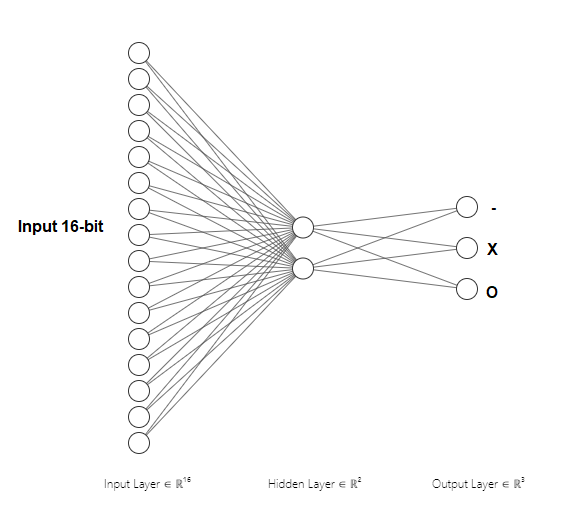
\includegraphics[width=1\linewidth, height=0.8\linewidth]{s1.png}
    \caption{Schemat sieci neuronowej}
\end{figure}
\subsection{Model sieci neuronowej}
\begin{lstlisting}[frame=single]
data = np.loadtxt("dane_do_MLP.txt")
train_label = []
train_data = []
tr_data = data
ts_data = data[int(0.9*len(data)):]
for item in tr_data:
    train_data.append(item[0:16])
    train_label.append(item[16])
test_data = []
test_label = []
for item in ts_data:
    test_data.append(item[0:16])
    test_label.append(item[16])

test_data = np.array(test_data, dtype=np.int8)
test_label = np.array(test_label, dtype=np.int8)
test_label = tf.keras.utils.to_categorical(test_label)

train_data = np.array(train_data, dtype=np.int8)
train_label = np.array(train_label, dtype=np.int8)
train_label = tf.keras.utils.to_categorical(train_label)

MLP = tf.keras.Sequential()
MLP.add(tf.keras.layers.InputLayer(input_shape=(16,)))
MLP.add(tf.keras.layers.Dense(2, activation='relu'))
MLP.add(tf.keras.layers.Dense(3, activation='softmax'))
MLP.compile(loss='categorical_crossentropy',
            optimizer='Adam',
            metrics=['accuracy'])
MLP.fit(train_data, train_label, epochs=35, batch_size=128)
out = MLP.get_weights()
np.savetxt("weight_1.txt",out[0])
np.savetxt("bias_1.txt",out[1])
np.savetxt("weight_2.txt",out[2])
np.savetxt("bias_2.txt",out[3])
\end{lstlisting}
\subsection{Model referencyjny}



\begin{lstlisting}[frame=single]
 def reference_module(input):
    weight_1 = np.loadtxt("weight_1.txt")
    bias_1 = np.loadtxt("bias_1.txt")
    weight_2 = np.loadtxt("weight_2.txt")
    bias_2 = np.loadtxt("bias_2.txt")
    input = np.array(input).reshape(16, 1)
    w1 = (input * weight_1).T
    w2 = (np.sum(w1, axis=1)).reshape(13,1)+bias_1.reshape(13,1)
    w3 = (w2*weight_2).T
    output = np.sum(w3, axis=1)+bias_2
    if output[0] > output[1]:
        return 'O'
    elif output[0] < output[1]:
        return 'X'
    else:
        return '-'
\end{lstlisting}
Umieszczona powyżej funkcja została napisana w języku programowania Python z wykorzystaniem biblioteki NumPy.W funkcji zostały użyte parametry otrzymane po wytrenowaniu sieci neuronowej, która została napisana przy użyciu biblioteki TensorFlow. Ta funkcja przyjmuje jako parametr wektor 16-bitowy i odpowiednio do jego wartości zwraca kółko, krzyżyk lub myślnik(oznacza to, że nie otzymaliśmy  ani kółka ani krzyżyka).

\subsection{Opisy scenariuszy testowych oraz dane testowe}

Dane testowe to zbiór wektorów 16-bitowych, które nie były wykorzystane podczas trenowania sieci neuronowej. 
Jednym ze scenariuszy testowych jest sprawdzenie czy nasz program działa poprawnie dla danych, które przewidywaliśmy podczas tworzenia programu. W naszym przypadku są to wektory, które są pozostałościami danych użytych do trenowania rozszerzone o wektory reprezentujące obrazy, które są zbliżone poziomem zaszumienia do docelowych. 
\newpage
\begin{figure}[htbp]
\centering
\begin{subfigure}{0.3\textwidth}
  \centering
  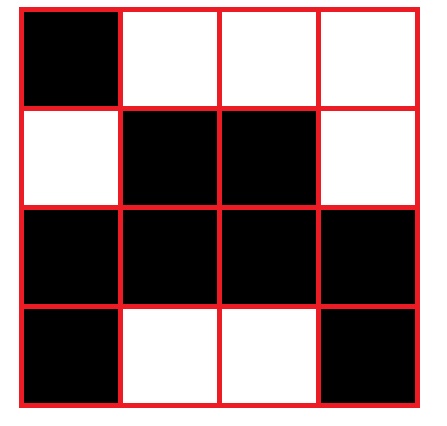
\includegraphics[width=\linewidth]{O.png}
  \label{fig:sub1}
\end{subfigure}
\begin{subfigure}{0,3\textwidth}
  \centering
  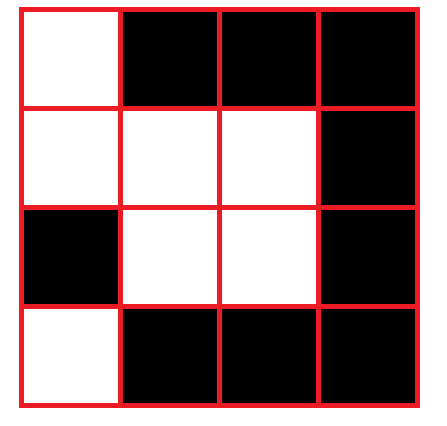
\includegraphics[width=\linewidth]{X.png}
  \label{fig:sub2}
\end{subfigure}
\begin{subfigure}{0,3\textwidth}
  \centering
  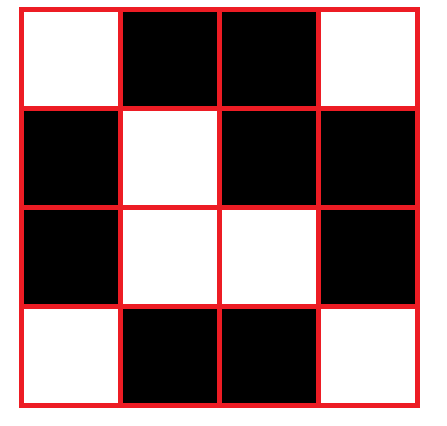
\includegraphics[width=\linewidth]{X1.png}
  \label{fig:sub3}
\end{subfigure}
\caption{Przykładowy wygląd obrazków w pierwszym scenariuszu testowym}
\label{fig:fig}
\end{figure}

Kolejnym scenariuszem jest wzięcie pod uwagę danych, przy których nie oczekujemy już poprawnych wyników, ale liczymy, że program wyłapie przypadki, w których mogą wystąpić sytuacje, które nie są możliwe do oceny. Ten przypadek jest nam potrzebny, aby odpowiednio reagować w ich przypadku.

\begin{figure}[htbp]
\centering
\begin{subfigure}{0.3\textwidth}
  \centering
  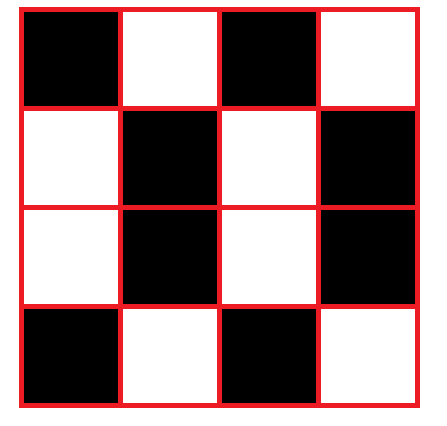
\includegraphics[width=\linewidth]{OX.png}
  \label{fig:sub1}
\end{subfigure}
\begin{subfigure}{0,3\textwidth}
  \centering
  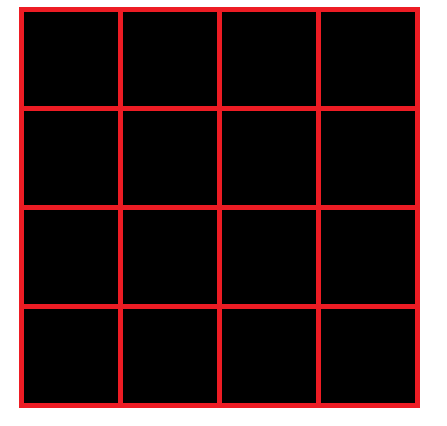
\includegraphics[width=\linewidth]{OX2.png}
  \label{fig:sub2}
\end{subfigure}
\begin{subfigure}{0,3\textwidth}
  \centering
  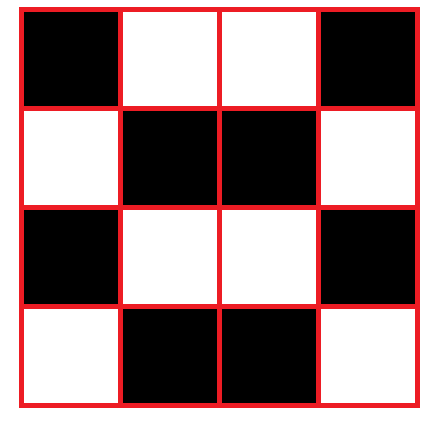
\includegraphics[width=\linewidth]{OX3.png}
  \label{fig:sub3}
\end{subfigure}
\caption{Przykładowy wygląd obrazków w drugim scenariuszu testowym}
\label{fig:fig}
\end{figure}
\newpage
\section{\large Etap IV}
\subsection{Sposób realizacji systemu}
\begin{lstlisting}
module proj( 
	input [15:0] in,
	output [1:0] out
);
reg signed [16:0] relu_1, relu_2;
reg signed [16:0] result_0,result_1,result_2;

localparam signed [7:0] weight_1_15_0 = 8'sb1111_0101;
localparam signed [7:0] weight_1_14_0 = 8'sb0000_1011;
localparam signed [7:0] weight_1_13_0 = 8'sb0000_1011;
localparam signed [7:0] weight_1_12_0 = 8'sb1111_0101;
localparam signed [7:0] weight_1_11_0 = 8'sb0000_1011;
localparam signed [7:0] weight_1_10_0 = 8'sb1111_0101;
localparam signed [7:0] weight_1_9_0 = 8'sb1111_0101;
localparam signed [7:0] weight_1_8_0 = 8'sb0000_1011;
localparam signed [7:0] weight_1_7_0 = 8'sb0000_1011;
localparam signed [7:0] weight_1_6_0 = 8'sb1111_0101;
localparam signed [7:0] weight_1_5_0 = 8'sb1111_0101;
localparam signed [7:0] weight_1_4_0 = 8'sb0000_1011;
localparam signed [7:0] weight_1_3_0 = 8'sb1111_0101;
localparam signed [7:0] weight_1_2_0 = 8'sb0000_1011;
localparam signed [7:0] weight_1_1_0 = 8'sb0000_1011;
localparam signed [7:0] weight_1_0_0 = 8'sb1111_0101;
localparam signed [7:0] weight_1_15_1 = 8'sb1110_1100;
localparam signed [7:0] weight_1_14_1 = 8'sb0001_0011;
localparam signed [7:0] weight_1_13_1 = 8'sb0001_0011;
localparam signed [7:0] weight_1_12_1 = 8'sb1110_1100;
localparam signed [7:0] weight_1_11_1 = 8'sb0001_0011;
localparam signed [7:0] weight_1_10_1 = 8'sb1110_1100;
localparam signed [7:0] weight_1_9_1 = 8'sb1110_1100;
localparam signed [7:0] weight_1_8_1 = 8'sb0001_0011;
localparam signed [7:0] weight_1_7_1 = 8'sb0001_0011;
localparam signed [7:0] weight_1_6_1 = 8'sb1110_1100;
localparam signed [7:0] weight_1_5_1 = 8'sb1110_1100;
localparam signed [7:0] weight_1_4_1 = 8'sb0001_0011;
localparam signed [7:0] weight_1_3_1 = 8'sb1110_1100;
localparam signed [7:0] weight_1_2_1 = 8'sb0001_0011;
localparam signed [7:0] weight_1_1_1 = 8'sb0001_0011;
localparam signed [7:0] weight_1_0_1 = 8'sb1110_1100;
localparam signed [7:0] weight_2_1_0 = 8'sb0010_1110;
localparam signed [7:0] weight_2_0_0 = 8'sb1101_0101;
localparam signed [7:0] weight_2_1_1 = 8'sb1111_1010;
localparam signed [7:0] weight_2_0_1 = 8'sb0100_0001;
localparam signed [7:0] weight_2_1_2 = 8'sb1001_1110;
localparam signed [7:0] weight_2_0_2 = 8'sb1111_0000;

localparam signed [7:0] bias_0 = 8'sb0011_0111;
localparam signed [7:0] bias_1 = 8'sb1110_0101;
localparam signed [7:0] bias_2 = 8'sb0000_0000;
localparam signed [7:0] bias_3 = 8'sb1100_0010;
localparam signed [7:0] bias_4 = 8'sb0010_1001;

always @(in) begin
	//hidden layer - feed forward from input to hidden layer
	relu_1 = bias_0 +$signed(in[0])*weight_1_0_0+$signed(in[1])*weight_1_1_0+
    $signed(in[2])*weight_1_2_0+$signed(in[3])*weight_1_3_0+
    $signed(in[4])*weight_1_4_0+$signed(in[5])*weight_1_5_0+
    $signed(in[6])*weight_1_6_0+$signed(in[7])*weight_1_7_0+
    $signed(in[8])*weight_1_8_0+$signed(in[9])*weight_1_9_0+
    $signed(in[10])*weight_1_10_0+$signed(in[11])*weight_1_11_0+
    $signed(in[12])*weight_1_12_0+$signed(in[13])*weight_1_13_0+
    $signed(in[14])*weight_1_14_0+$signed(in[15])*weight_1_15_0;
	
	relu_2 = bias_1+$signed(in[0])*weight_1_0_1+$signed(in[1])*weight_1_1_1+
    $signed(in[2])*weight_1_2_1+$signed(in[3])*weight_1_3_1+
    $signed(in[4])*weight_1_4_1+$signed(in[5])*weight_1_5_1+
    $signed(in[6])*weight_1_6_1+$signed(in[7])*weight_1_7_1+
    $signed(in[8])*weight_1_8_1+$signed(in[9])*weight_1_9_1+ 
    $signed(in[10])*weight_1_10_1+$signed(in[11])*weight_1_11_1+
    $signed(in[12])*weight_1_12_1+$signed(in[13])*weight_1_13_1+
    $signed(in[14])*weight_1_14_1+$signed(in[15])*weight_1_15_1;
	//hidden layer - activation function - ReLU
	relu_1 = relu_1>1'sb0 ? relu_1:1'sb0;
	relu_2 = relu_2>1'sb0 ? relu_2:1'sb0;
	//output
	result_0 = relu_1*weight_2_1_0+relu_2*weight_2_0_0+bias_2;
	result_1 = relu_1*weight_2_1_2+relu_2*weight_2_0_2+bias_4;
	result_2 = relu_1*weight_2_1_1+relu_2*weight_2_0_1+bias_3;
end

assign out = result_0>=result_1 ? (result_0>=result_2 ? 2'b00:2'b10)
:(result_1>=result_2 ? 2'b01:2'b10);

endmodule

\end{lstlisting}
\captionof{lstlisting}{Implementacja w języku Verilog HDL}
Zgodnie z planowanym modelem zaimportowaliśmy sieć neuronową, która została wcześniej wytrenowana. Przy pomocy odpowiednich współczynników wyeksportowanych z tego modelu, zaimplementowaliśmy tą sieć. Pierwszym krokiem była zamiana współczynników na liczby w formacie stałoprzecinkowym. Dla uzyskanych liczb był to format (4,4), czyli 4 bity przed przecinkiem i 4 bity po przecinku, gdyż dla takich wartości utrzymaliśmy taką samą dokładność wyników co dla większej ilości bitów po przecinków. W przypadku 3 lub mniej bitów po przecinków zaczęły pojawiać błędne wyniki. Po ustawieniu wartości wszystkich parametrów, policzyliśmy przejście pomiędzy warstwami i wartość po zastosowaniu funkcji aktywacji neuronu. W ostatniej części uzyskane wartości obu neuronów przekazujemy do kolejnej warstwy i otrzymujemy 3 wartości odpowiadające każdemu z wyjść. Jako iż napisanie funkcji softmax w języku Verilog jest dość dużym wyzwaniem, skorzystaliśmy z przybliżenia za pomocą zagnieżdżenia operatora trójargumentowego. Podany kod zwraca wartość w zakresie od 0 do 2, gdzie 0 oznacza brak rozwiązania, 1 oznacza kółko i 2 oznacza krzyżyk.
\subsection{Symulacja i ocena rozwiązania}
Sprawdziliśmy poprawność działalności (czyli poprawność wykrycia znaków "X" i "O") powyżej zaimplementowanej sieci z pomocą RTL symulacji. Do testowania wykorzystaliśmy zestaw danych testowych(wszystkie możliwe 16-bitowe wektory). Na wyjściu otrzymaliśmy 3 róźne wartości: 2 i 1, gdy sieć rozpoznaje "X" lub "O" odpowiednio oraz 0, gdy wektor wejściowy nie pasuje do żadnego z poszukiwanych symboli.
Możemy stwierdzić że dostaliśmy prawie 95\% subiektywnie dobrych wyników, co świadczy o tym, że nasz program działa poprawnie. 
Poza tym, czas propagacji wynosi 1 pikosekunde, co jest stosunkowo mało, więc można stwierdzić, że nasze rozwiązanie jest optymalne.
\newpage
\begin{figure}[h]
    \centering
    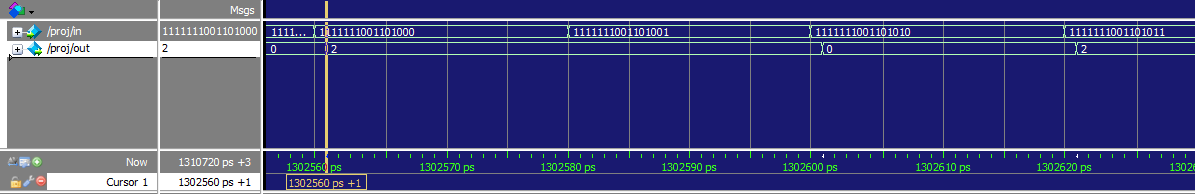
\includegraphics[width = \textwidth]{czas_propagacji.png}
    \caption{Czas propagacji}
    \label{fig:my_label}
\end{figure}
\begin{figure}[h]
    \centering
    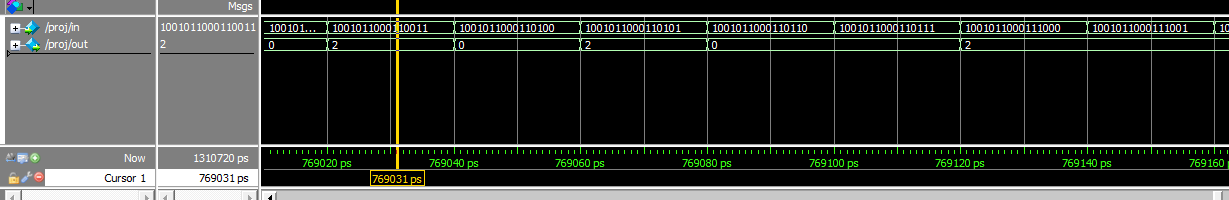
\includegraphics[width = \textwidth]{sym1.png}
    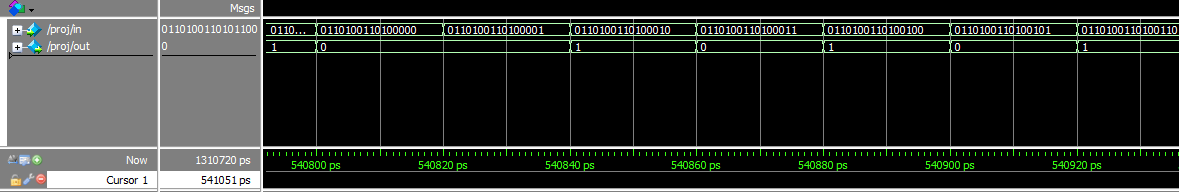
\includegraphics[width = \textwidth]{sym2.png}
    \caption{Wyniki symulacji}
    \label{fig:my_label}
\end{figure}

\subsection{Testbench}
\begin{lstlisting}
from vcdvcd import VCDVCD
import numpy as np
vcd_file = "dane_symulacji.vcd"
vcd_data = VCDVCD(vcd_file)
text_file = open("dane_testowe.txt", "r")
text_lines = text_file.readlines()
text_file.close()
out_1 = vcd_data.data['1'].tv[1:]
out_0 = vcd_data.data['2'].tv[1:]


def sampling(input):
    sampled_data = []
    interval = 20
    end_time = input[-1][0]
    current_time = 0
    current_value = None
    data_index = 0

    while current_time <= end_time:
        if data_index < len(input) and current_time >= input[data_index][0]:
            current_value = input[data_index][1]
            data_index += 1

        sampled_data.append((current_time, current_value))
        current_time += interval
    return sampled_data

out = []
out_1 = sampling(out_1)
out_0 = sampling(out_0)
test_output = []
counter = 0
for i in range(2**16):
    out.append(out_1[i][1]+out_0[i][1])
for i in range(len(text_lines)):
    text_lines[i] = text_lines[i].strip()
    test_output.append(np.binary_repr(int(text_lines[i][-1]),2))
counter_val = 0
for i in range(len(test_output)):
    if not out[i] == test_output[i]:
        counter = counter +1
        if test_output[i]=='00':
            counter_val = counter_val+1
print(counter, counter_val)
\end{lstlisting}
\captionof{lstlisting}{Plik testowy}
Powyższy kod został użyty do sprawdzenia poprawności rozwiązania. Z powodu problemów z napisaniem testbencha, zaimportowaliśmy dane z symulacji Modelsim i poprzez podany kod spróbkowaliśmy dane z pliku o formacie .vcd. Dane uzyskane w ten sposób porównywaliśmy z ich odpowiednikami wygenerowanymi na potrzeby trenowana sieci neuronowej. Ostatnia pętla for zlicza różnice pomiędzy tymi danymi i przechowuje tą wartość w zmiennej counter. Po sprawdzeniu wszystkich danych otrzymaliśmy wartość pierwszego licznika. Drugi licznik - counter\_val zlicza ilość przypadków, dla których teoretycznie powinien być brak rozwiązania, ale jest wykryte kółko lub krzyżyk. Okazało się, że wszystkie 1820 błędnych wyników jest zamienionym 0 na 1 lub 2. Po przejrzeniu tych danych duża ich część różni się 4-ma pikselami, czyli jest to dla nas wartość dopuszczalna i możemy przyjąć, że pomimo tych błędów rozwiązanie jest dokładne.





\newpage
\section{\large Etap V}
% W tym etapie należy opisać uruchomienie systemu na docelowej platformie(Etap V)

Jako docelową platformę do zrealizowania oraz przetestowania naszego projektu zdecydowalismy się wybrać Logisim Evolution. Później przetestowaliśmy działanie naszej sieci neuronowej również na płytce laboratoryjnej DE2-115.

\subsection{Realizacja sieci neuronowej w Logisim Evolution}
Realizację rozpoczeliśmy od dodania 16-tu 16-bitowych pinów wejściowych (in) oraz 2-bitowego wyjściowego (out).

\begin{figure}[h]
\centering
    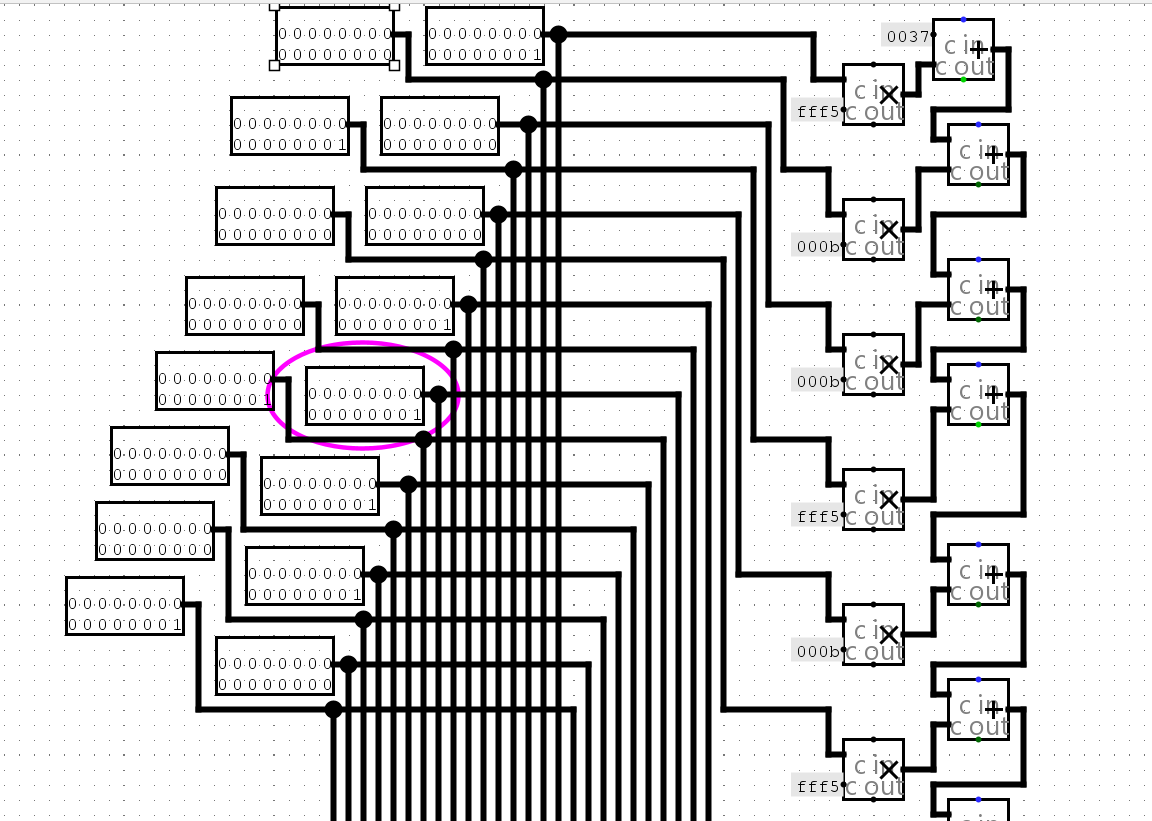
\includegraphics[width=0.8\linewidth]{Inputs.png}
    \caption{Wejścia oraz komponenty Multiplier i Adder}
\end{figure}

Następnie, stworzyliśmy wagi dodając 16-bitowe wartości stałe(constanty) po czym przypisaliśmy do nich odpowiedne wartości.
\newline
Kolejnym krokiem było dodanie komponentu mnożenia (Multiplier) do wyliczania relu\underline{ }1 oraz relu\underline{ }2. Aby tego dokonać potrzebowaliśmy osobnej mnożarki dla każdej operacji mnożenia w Verilog'u. Podłączyliśmy odpowiednią stałą do jednego wejścia mnożnika, a odpowiedni bit zmiennej 'in' do drugiego wejścia.  
\newline
Po realizacji wszystkich mnożarek, dodawaliśmy komponenty Adder do sumowania wszystkich zmnożonych wartości. Na końcu dostawaliśmy odpowiednio wartości relu\_1 oraz relu\_2.
\newpage

Dalej użyliśmy komponentu dodawania aby zsumować wyniki operacji mnożenia. Przy pomocy tego komponentu obliczyliśmy relu\_1 oraz relu\_2.
\newline
Funckję ReLU zaimplementowaliśmy za pomocą komparatora i multipleksera. Jeżeli wartość będzie większa niż zero to na wyjściu emitujemy wartość wejściową.
W przeciwnym przypadku emitujemy zero. Realizacja ma działać tak dla  relu\_1 oraz relu\_2.

\begin{figure}[h!]
\centering
    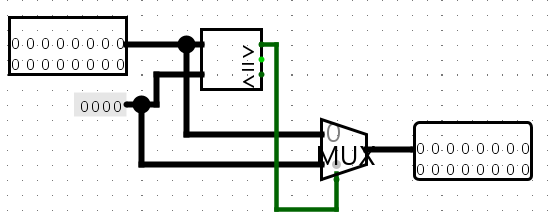
\includegraphics[width=0.8\linewidth]{Relu.png}
    \caption{Funckja ReLU}
\end{figure}

Na koniec dodaliśmy drugą warstwę - warstwę mnożenia i dodawania z wynikami ReLU jak i  wagami drugiej warstwy aby móc obliczyć result\_0, result\_1 i result\_2.
\begin{figure}[h!]
\centering
    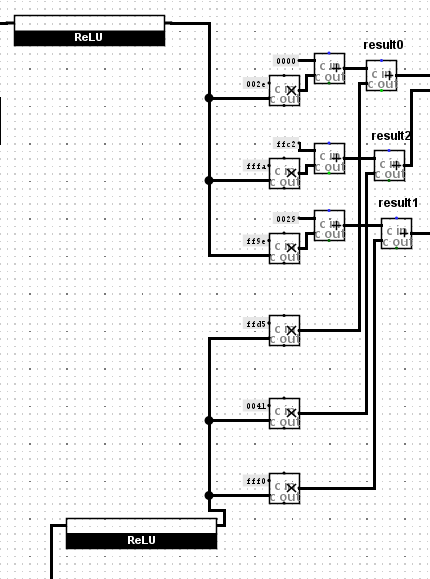
\includegraphics[width=0.5\linewidth]{Result.png}
    \caption{Otrzymanie trzech zmiennych result\_0, result\_1 oraz result\_2, które będą użyte do policzenia wyniku końcowego}
\end{figure}

\newpage
Użyliśmy komparatorów oraz multiplekserów do zaimplementowania logiki przypisania wyjścia, która wybiera odpowidnią wartość out na podstawie result\_0, result\_1 oraz result\_2.

\begin{figure}[h]
\centering
    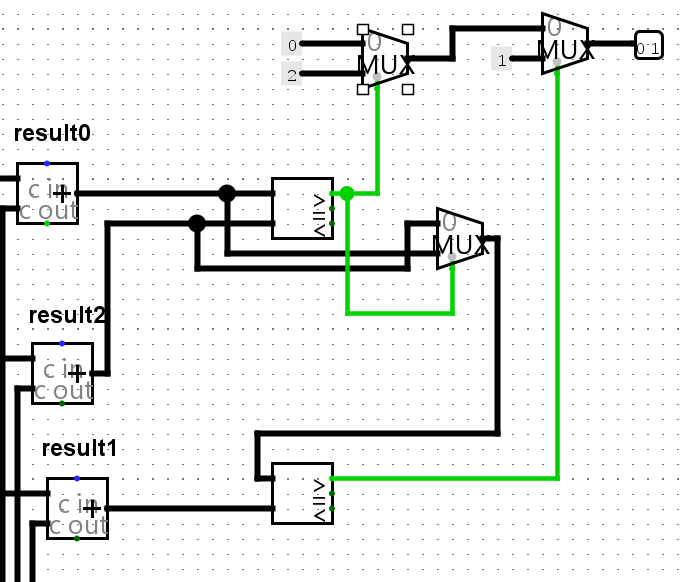
\includegraphics[width=0.7\linewidth]{Out.png}
    \caption{Ostatni etap do otrzymania wyniku końcowego}
\end{figure}

Po imtlementacji tej sieci w Logisimie, robiliśmy kilka testów. Testowaliśmy wartości wejściowe, odpowadające idealnym kółku i krzyżyku oraz zniekształconym kółku i krzyżyku. Nasza sieć działa poprawnie, ponieważ optrzymaliśmy te wartości na które spodziewaliśmy się( dla kółka to jest 2, a dla krzyżyka - 2). Także wartości zniekształconych znaków(czyli do 3-ch pikseli różnicy od znaku idealnego) są takie same, jak dla idealnych symboli.
\newpage
\subsection{Uruchomienie sieci neuronowej na płytce DE2-115}
Nasze rozwiązanie problemu projektowego postanowiliśmy uruchomić na płytce DE2-115.\newline
Najpierw utworzyliśmy projekt w Quartus'ie i skompilowaliśmy go.
Następnie odpowiednio ustawiliśmy piny w narzędziu Pin Planner. Bity inputu 0-15 umieściliśmy odpowiednio na przełącznikach \emph{sw15, sw14, ..., sw0}. Outputy umieściliśmy na czerwonych diodach \emph{ledr}. Po ustawienu pinów uruchomiliśmy płytkę.\newline

\begin{figure}[h!]
    \centering
    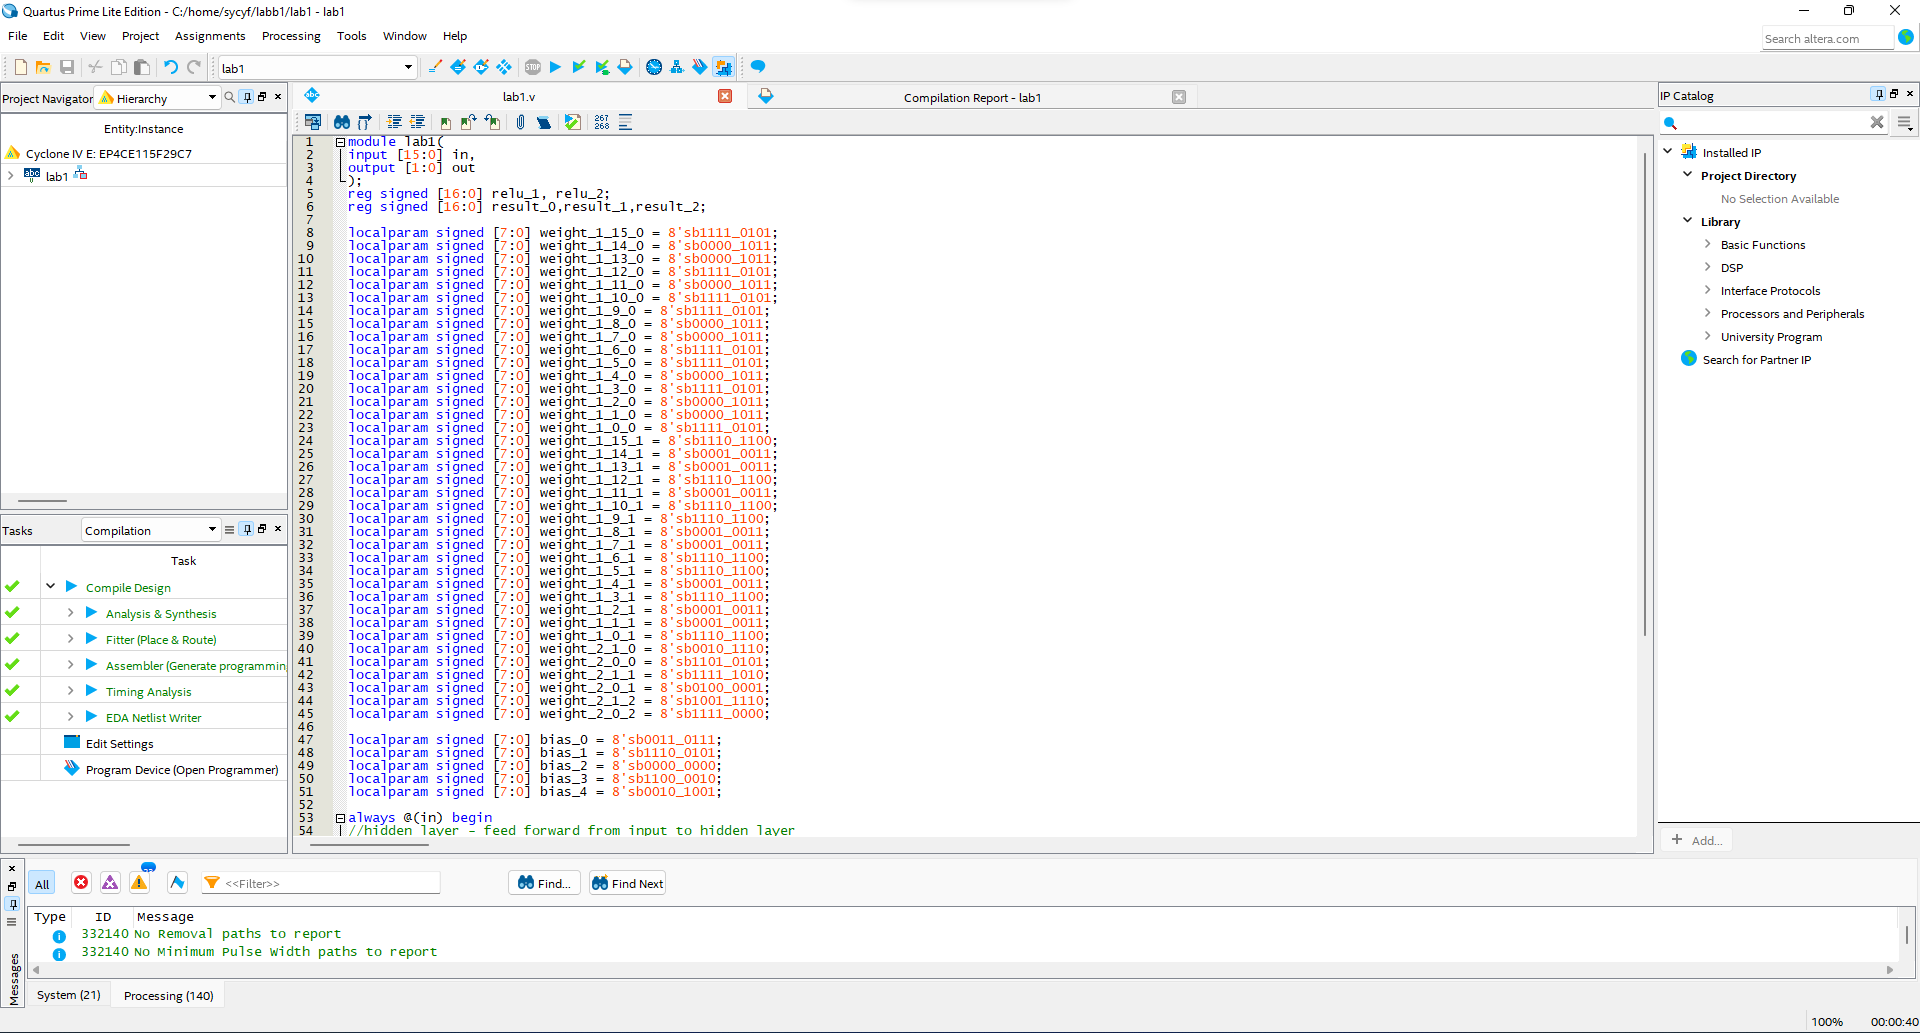
\includegraphics[width = 0.9\textwidth]{code.png}
    \caption{Fragment kodu, opisującego działanie naszej sieci neuronowej}
    \label{fig:enter-label}
\end{figure}
\begin{figure}[h!]
    \centering
    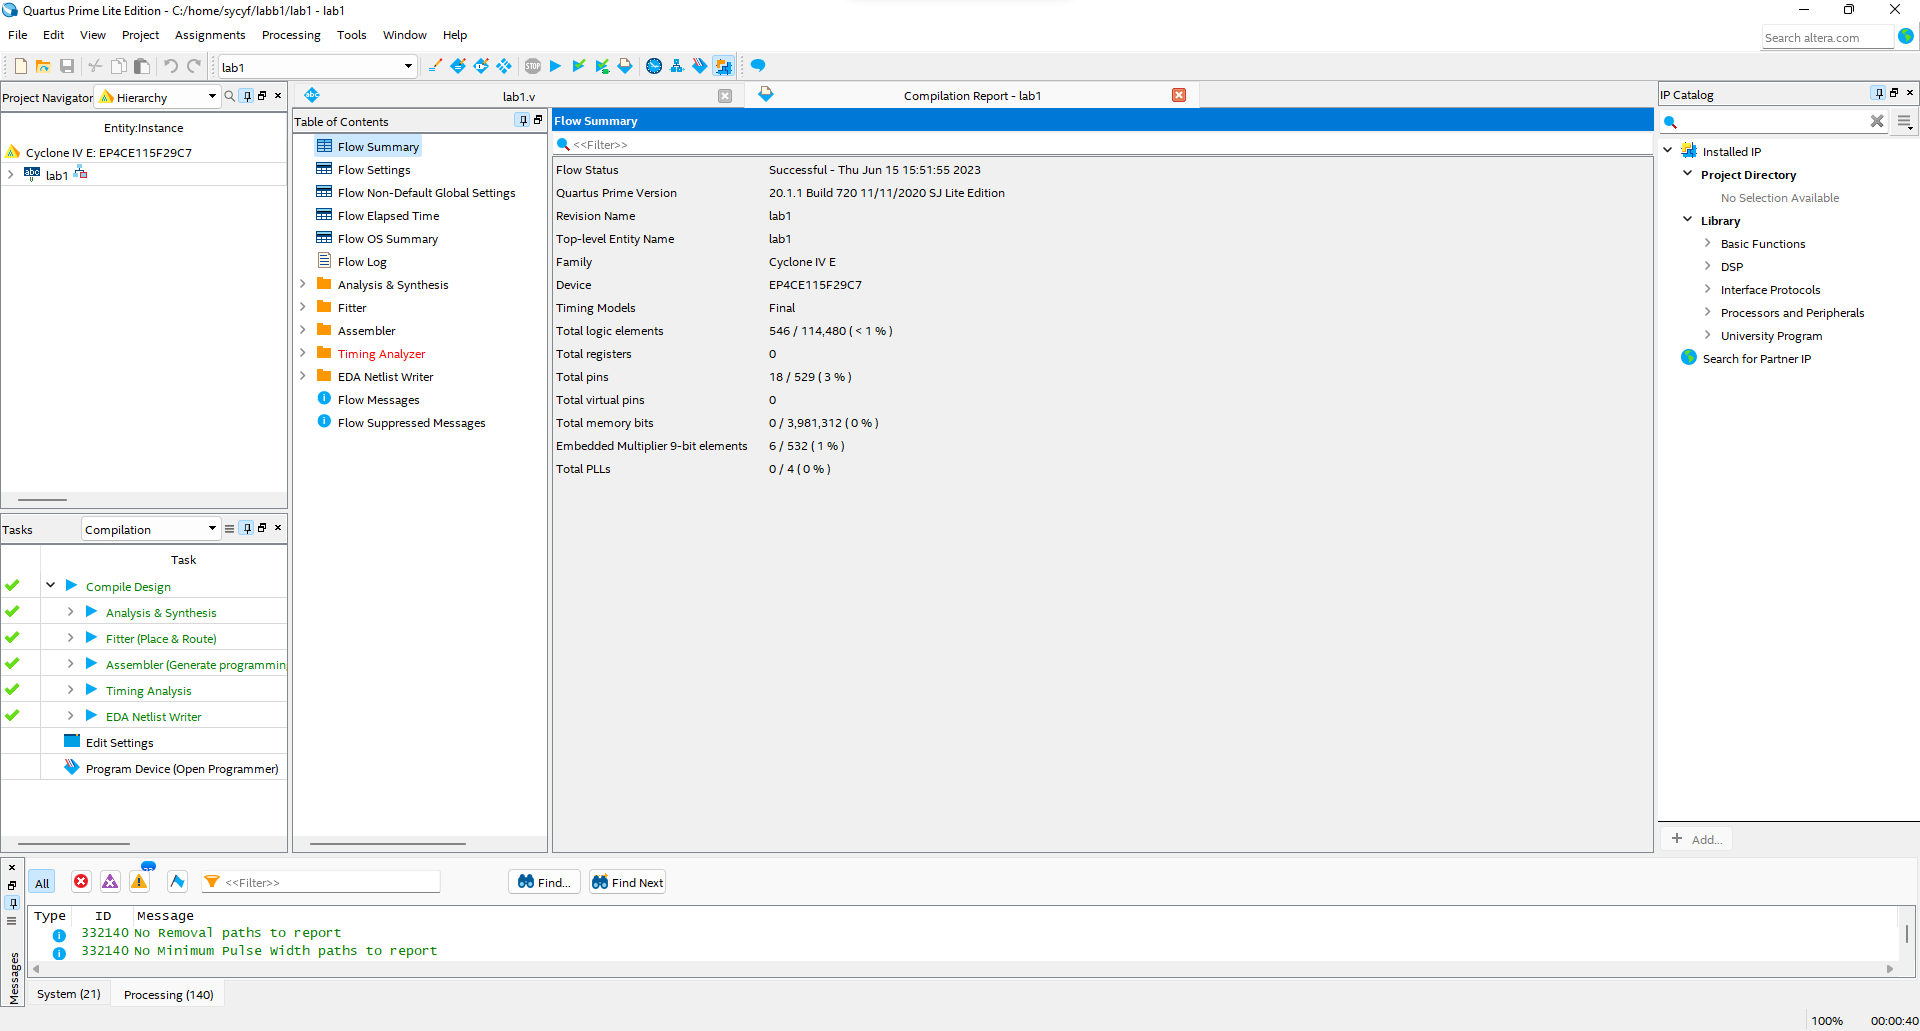
\includegraphics[width = 0.9\textwidth]{compilation.png}
    \caption{Wyniki kompilacji}
    \label{fig:enter-label}
\end{figure}
\newpage
\begin{figure}[h!]
    \centering
    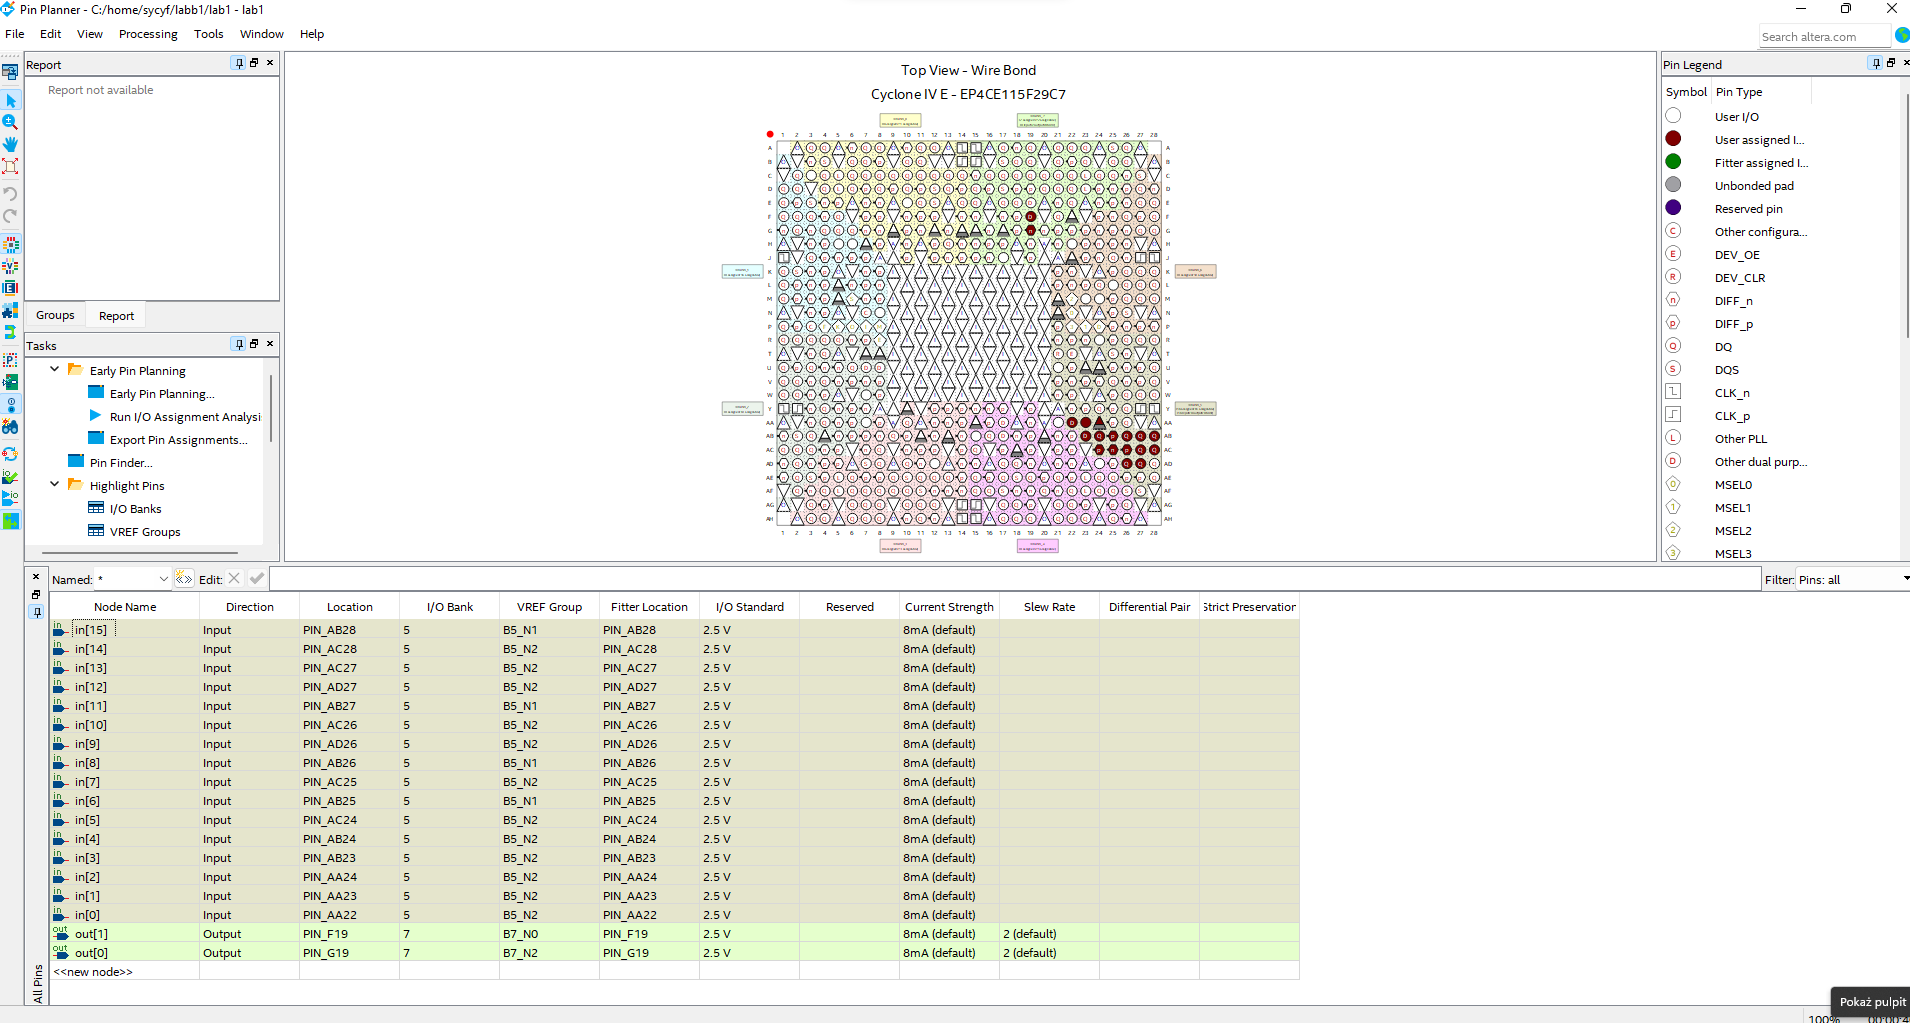
\includegraphics[width = 0.9\textwidth]{pins.png}
    \caption{Ustawienie pinów}
    \label{fig:enter-label}
\end{figure}
\begin{figure}[h!]
    \centering
    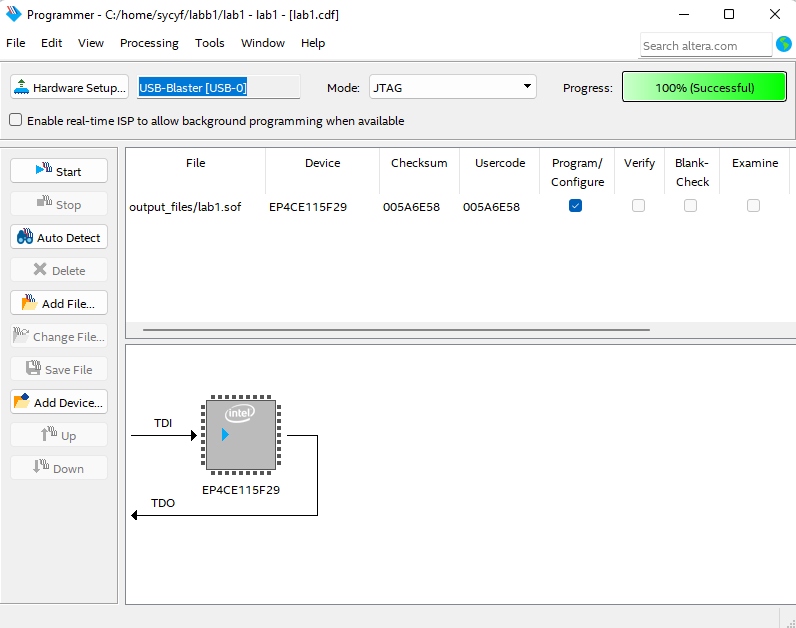
\includegraphics[width = 0.8\textwidth]{programmer.png}
    \caption{Okienko programmera}
    \label{fig:enter-label}
\end{figure}
Po odpaleniu płytki w pierwszej kolejności sprawdziliśmy poprawność działania sieci w przypadku wystąpienia idealnego krzyżyka oraz kółka. Potem sprawdzaliśmy zachowanie naszej sieci kiedy na wejściu otrzymujemy zniekształcone znaki. Na koniec ustawiliśmy dane wejściowe, których system nie rozpoznaje  ani jako kółko ani krzyżyk. Wszystkie testy zakończyły się pomyślnie, zatem sieć działa zgodnie z oczekiwaniami.
\begin{figure}[h!]
    \centering
    \includegraphics[width = \textwidth, height = 0.6\textwidth]{idealny_krzyż.jpg}
    \caption{Rozpoznawanie idealnego krzyżyka}
    \label{fig:enter-label}
\end{figure}
\begin{figure}[h!]
    \centering
    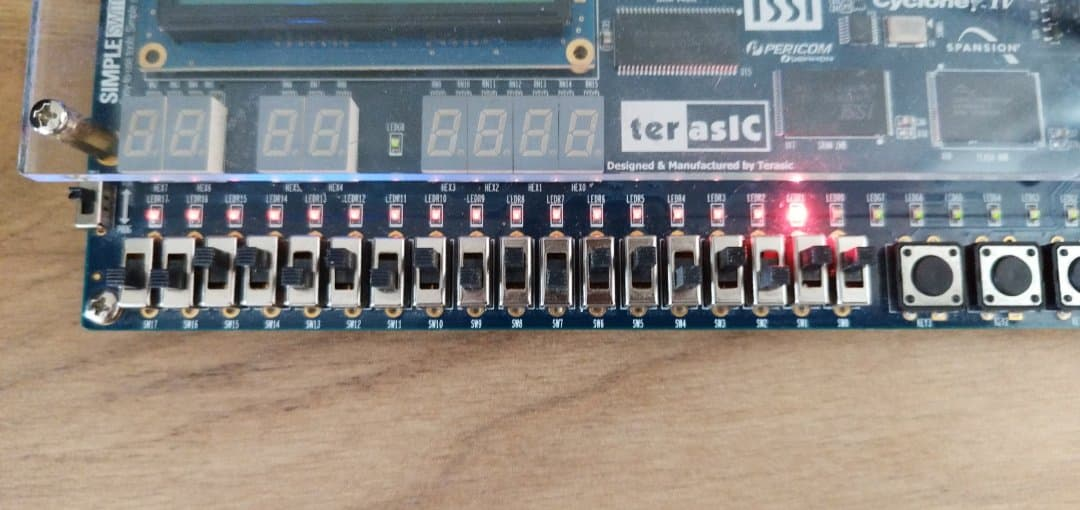
\includegraphics[width = \textwidth, height = 0.6\textwidth]{zniekształcony_krzyż.jpg}
    \caption{Rozpoznawanie zniekształconego krzyżyk}
    \label{fig:enter-label}
\end{figure}
\begin{figure}[h!]
    \centering
    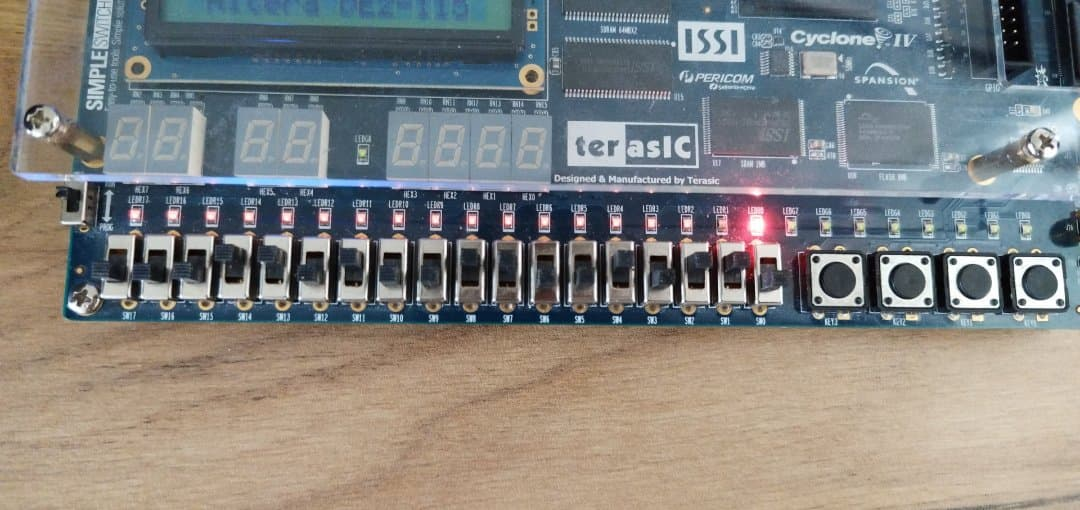
\includegraphics[width = \textwidth, height = 0.6\textwidth]{idealne_kółko.jpg}
    \caption{Rozpoznawanie idealnego kółka}
    \label{fig:enter-label}
\end{figure}
\begin{figure}[h!]
    \centering
    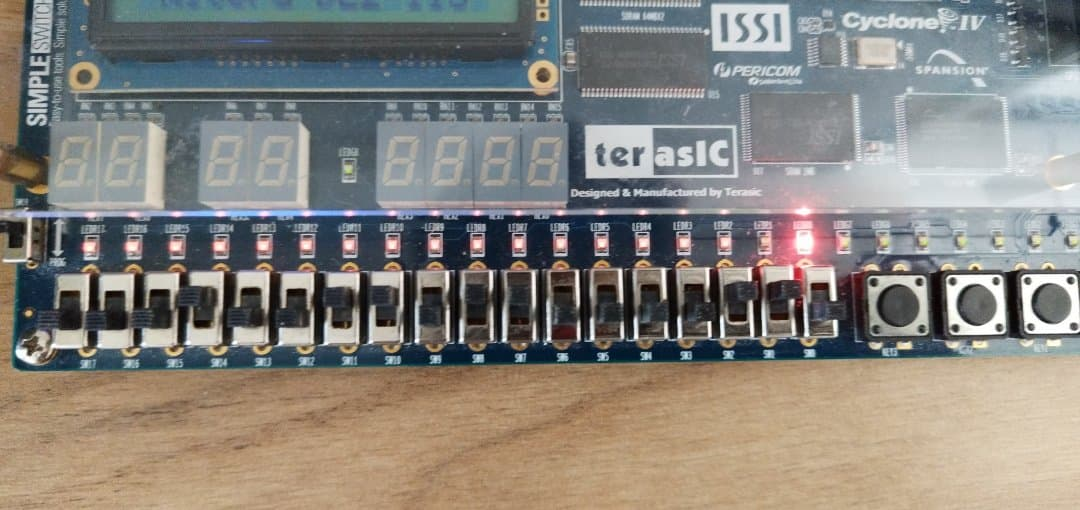
\includegraphics[width = \textwidth, height = 0.6\textwidth]{zniekształcone_kółko.jpg}
    \caption{Rozpoznawanie zniekształconego kółka}
    \label{fig:enter-label}
\end{figure}
\begin{figure}[h!]
    \centering
    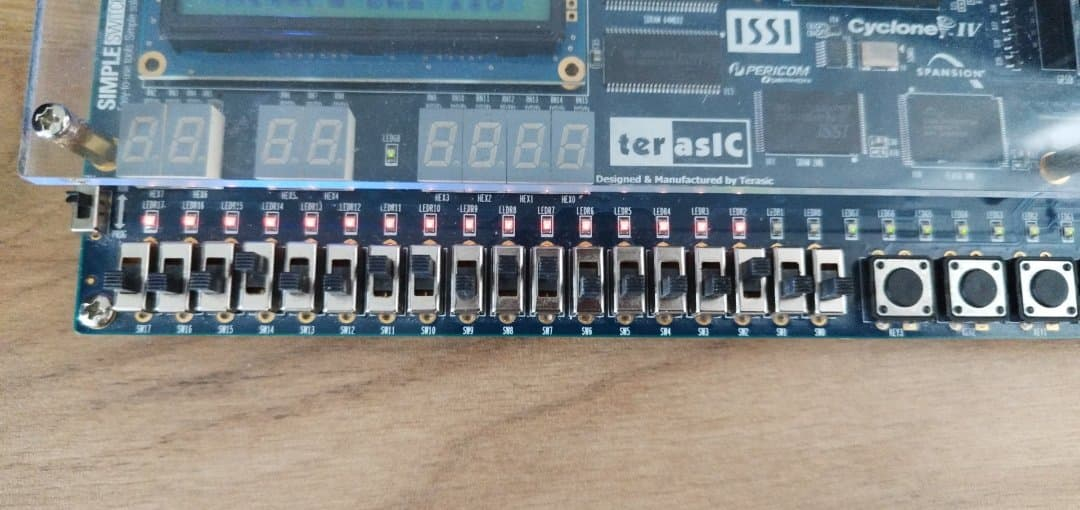
\includegraphics[width = \textwidth, height = 0.6\textwidth]{nic1.jpg}
    \caption{Sieć nie rozpoznaje znaku(1)}
    \label{fig:enter-label}
\end{figure}
\begin{figure}[h!]
    \centering
    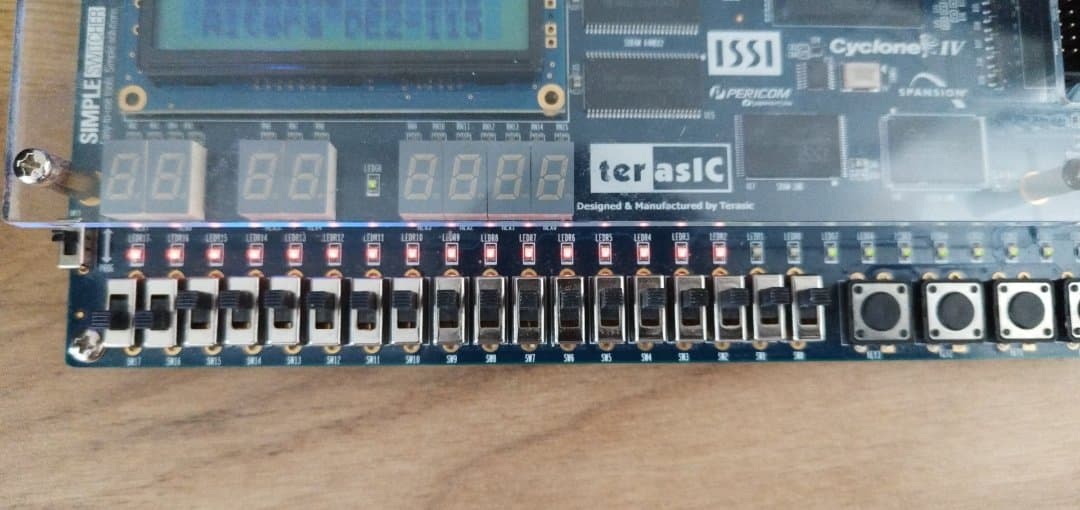
\includegraphics[width = \textwidth, height = 0.6\textwidth]{nic2.jpg}
    \caption{Sieć nie rozpoznaje znaku(2)}
    \label{fig:enter-label}
\end{figure}

\section{\Large{Literatura}}
\begin{itemize}
    \item \label{1}[1] Model LeNet-5 - \url{https://towardsdatascience.com/understanding-and-implementing-lenet-5-cnn-architecture-deep-learning-a2d531ebc342}
    \item \label{2}[2] Model ResNet - \url{https://datascience.eu/pl/uczenie-maszynowe/przeglad-sieci-resnet-i-jej-wariantow/}
    \item \label{3}[3] Metoda k-najbliższych sąsiadów (k-NN) - \url{https://www.statsoft.pl/textbook/stathome_stat.html?https://www.statsoft.pl%2Ftextbook%2Fstknn.html}
    \item \label{4}[4] SVM - \url{https://home.agh.edu.pl/~horzyk/lectures/miw/MIW-SVM.pdf}
    \item \label{5}[5]Template Matching in Binary Images - Miguel Velhote Correia - \url{https://www.researchgate.net/publication/268815275_Template_Matching_in_Binary_Images}
\end{itemize}
\end{document}